% https://tex.stackexchange.com/a/482806
\documentclass{beamer}

\usepackage{tikz}
\usetikzlibrary{overlay-beamer-styles}

\begin{document}

\begin{frame}
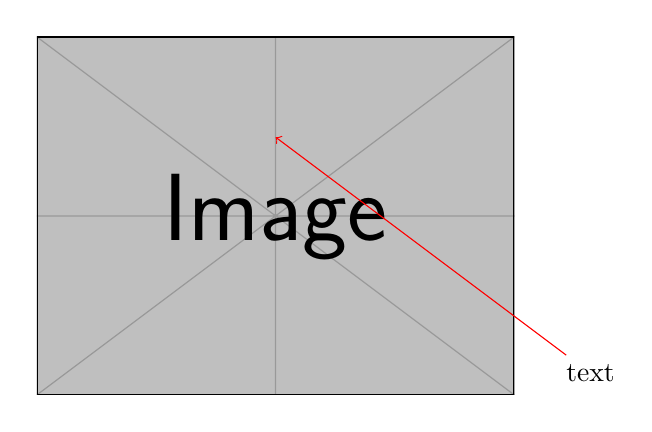
\begin{tikzpicture}
\node {\includegraphics[width=.5\textwidth]{example-image}};
\node[visible on=<2>] (a) at (4,-2) {text};
\draw[<-,red,visible on=<2>] (0,1) -- (a);
\end{tikzpicture}
\end{frame}

\end{document}
